\lecture{19}{2020-07-15}{Exploration (Part 2)}

\subsubsection{Muestreo de Thompson}%
\label{ssub:muestreo_de_thompson}

Se aprende una distribución sobre las funciones Q o las políticas y se muestrea y actúa de
acuerdo con las muestras extraídas.

\begin{align}
    \theta_1, \ldots,\theta_n\sim \hat{p}(\theta_1,\ldots,\theta_n)\\
    a=arg\max_a E_{\theta_a}[r(a)]
\end{align}

En el problema de los \textit{bandits} se mantenía una distribución del modelo (se muestrea
lo que se piensa que va a dar el entorno). En un problema de DRL una opción es que representen
la distribución de las funciones Q.

Lo teóricamente correcto si se quiere hacer un muestreo de Thompson en un problema de DRL es
tener una distribución sobre el MDP. En la práctica esto es complicado por lo que se suele
hacer la distribución sobre las funciones Q, que son un análogo del MDP.

Lo siguiente, repetido, describe un proceso de RL
\begin{enumerate}
    \item Se muestrea la función Q a partir de $p(Q)$
    \item Se actúa según $Q$ por un episodio.
    \item Actualizar $p(Q)$
\end{enumerate}
Esto se puede hacer con Q-Learning porque es off-policy, si se quieren usar PG la cosa se
complica más.

\subsubsection{Ganancia de información}%
\label{ssub:ganancia_de_información}

Se razona sobre la ganancia de información desde la visita a nuevos estados.

La intuición dice de usar IG con respecto a la recompensa, pero en la práctica se suelen
tener entornos con una recompensa muy dispersa por lo que esto no funciona.

Una opción que funciona mejor es medir IG en función de la densidad de $p(s)$.
Intuitivamente esto hace que se elijan acciones que cambien nuestras creencias sobre
$p(s)$.

Otra opción es considerar IG sobre la dinámica  $p(s'|s,a)$.

Generalmente esto no es tratable en la práctica, sea lo que sea lo que se esté estimando, por
lo que se trabajará con aproximaciones. Se pueden elegir varias aproximaciones:
 \begin{itemize}
     \item Ganancia de predicción (\textit{prediction gain}): se define como $\log
         p_{\theta'}(s)-\log p_{\theta'}(s)$. Es muy parecido a IG matemáticamente.
         $\theta'$ son los parámetros actualizados después de visitar $s$. Intuitivamente, si
         la densidad cambia mucho es que el estado era nuevo. 
     \item Inferencia variacional (Houthooft et al. "VIME"): IG se puede escribir de forma
         equivalente como $D_{KL}(p(z|y)||p(z))$. Se puede aprender las recompensas o las
         funciones Q pero de ejemplo se va a mostrar como aprender las transiciones
         $p_\theta(s_{t+1}|s_t,a_t):\;\;z=\theta$. Lo que se observa es
         $y=(s_t,a_t,s_{t+1})$. Como se sabe que IG es equivalente a la divergencia KL, se
         sustituye por la definición de  $z$ y $\theta$:
         \begin{align}
             D_{KL}(p(\theta|h,s_t,a_t,s_{t+1})||p(\theta|h))
         \end{align}
         La intuición está en que una transición es más informative si hace que el conocimiento
         sobre $\theta$ cambie. Como se dijo antes, esto no es tratable en la práctica por
         lo que se va a hacer una aproximación $q(\theta|\phi)\approx
         p(\theta|h)$, como por ejemplo inferencia variacional. Por lo que ahora dada una
         transición nueva $(s,a,s')$, se actualiza $\phi$ para conseguir $\phi'$.
         Específicamente, se está optimizando la cota inferior variacional de
         $D_{KL}(q(\theta|\phi)||p(h|\theta)p(\theta))$.\\
         Se representa $q(\theta|\phi)$ como el producto de distribuciones gaussianas
         independientes con media $\phi$.
\end{itemize}

Como resumen final, IG tiene como ventaja su formalismo matemático pero por otra parte los
modelos son más complejos y difíciles de usar de forma efectiva ya que se tienen muchos
hiperparámetros.

\subsubsection{Lecturas recomendadas}%
\label{ssub:lecturas_recomendadas}

\begin{itemize}
    \item Schmidhuber. (1992). A Possibility for Implementing Curiosity and Boredom in Model-Building Neural Controllers.
    \item Stadie, Levine, Abbeel (2015). Incentivizing Exploration in Reinforcement Learning with Deep Predictive Models.
    \item Osband, Blundell, Pritzel, Van Roy. (2016). Deep Exploration via Bootstrapped DQN.
    \item Houthooft, Chen, Duan, Schulman, De Turck, Abbeel. (2016). VIME: Variational Information Maximizing Exploration.
    \item Bellemare, Srinivasan, Ostroviski, Schaul, Saxton, Munos. (2016). Unifying Count-Based Exploration and Intrinsic Motivation.
    \item Tang, Houthooft, Foote, Stooke, Chen, Duan, Schulman, De Turck, Abbeel. (2016). Exploration: A Study of Count-Based Exploration for Deep Reinforcement Learning.
    \item Fu, Co-Reyes, Levine. (2017). EX2: Exploration with Exemplar Models for Deep Reinforcement Learning.
\end{itemize}

\section{Aprendizaje por Imitación vs. Aprendizaje por refuerzo}%
\label{sec:aprendizaje_por_imitación_vs_aprendizaje_por_refuerzo}

\begin{center}
    \begin{tabular}{c | c}
    Imitación & RL\\
    \hline
    - Requiere demostraciones & - Requiere función de recompensa\\
    - \textit{Distributional shift} & - Exploración\\
    + Simple, estable y supervisado & - Potencialmente no convergente\\
    - Solamente tan bueno como la demostración & + Puede ser arbitrariamente bueno
    \end{tabular}
\end{center}

Interesa conseguir lo mejor de los dos mundos. Por ejemplo, ¿qué pasaría si se tienen
demostraciones y recompensas?

Una de las formas más sencillas de usar ambas es preentrenar con las imitaciones y ajustar el
agente resultante con las recompensas. Esto puede funcionar muy bien porque las
demostraciones evitan que se pierda tiempo en la exploración y RL puede mejorar la efectividad
por encima de la del demostrador.

\begin{algorithm}
    \caption{Preentrenar y ajustar}
    Recoger datos de demostraciones $(s_i,a_i)$ \\
    Inicializar $\pi_\theta$ como
    $\max_\theta\sum_i\log\pi_\theta(a_i|s_i)$ \\
    \Repeat{se converja}{
        Ejecutar $\pi_\theta$ para recoger experiencia\\
        Mejorar $\pi_\theta$ con cualquier algoritmo RL
    }
\end{algorithm}

El algoritmo anterior puede no funcionar ya que se puede coger lo peor de los dos mundos. Es
posible que se produzca el \textit{distributional shift} en el primer paso y que después la
política sea demasiado determinista como para explorar estados nuevos.

Si se tiene el primer batch de observaciones generadas que sean malas, puede destruir la
inicialización hecha previamente.

Una de las cosas que se puede hacer para solucionar esto es usar un algoritmo
\textit{off-policy}, de forma que se pueda entrenar sobre las demostraciones en cada
iteración.

\subsubsection{Policy Gradient con demostraciones}%
\label{ssub:policy_gradient_con_demostraciones}

Se incluyen muestras del demostrador en el dataset $D$. Aunque en $D$ para Policy Gradient se
ponían observaciones \textit{on-policy}, poner demostraciones no es mala idea debido al IS
óptimo, que se basa en que si se quiere calcular $E_{p(x)}[f(x)]$, la $q(x)$ que da la menor
varianza es $q(x)\propto p(x)|f(x)|$. 

Problemas:
\begin{itemize}
    \item ¿De qué distribución vienen las demostraciones?
        \begin{itemize}
            \item Opción 1: usar clonado de comportamiento supervisado para aproximar
                $\pi_{demo}$. No será una estimación buena pero será suficiente.
            \item Opción 2: Se asume una distribución del tipo delta de Dirac:
                $\pi_{demo}(\tau)= \frac{1}{N} \delta (\tau\in D)$.  Esto funciona mejor con
                IS autonormalizado (suma hasta 1): 
                \begin{align}
                    E_{p(x)}[f(x)]\approx \frac{1}{\sum_j \frac{p(x_j)}{q(x_j)} }
                    \sum_i \frac{p(x_i)}{q(x_i)} f(x_i)
                \end{align}
        \end{itemize}
    \item ¿Qué hacer si $D$ viene de múltiples distribuciones? IS sólo funciona para una
        distribución, si se quiere hacer esto de manera correcta se tiene que usar una
        \textit{fusion distribution}: $q(x)= \frac{1}{M} \sum_i q_i(x)$
\end{itemize}

\subsubsection{Q-Learning con demostraciones}%
\label{ssub:q_learning_con_demostraciones}

Es bastante fácil hacerlos funcionar con demostraciones ya que estas simplemente se meten en
el buffer, pero hay que gestionar algunas cosas.

Q-Learning ya es \textit{off-policy} por lo que no hay que preocuparse con los pesos.

\subsubsection{Problemas con estos planteamientos}%
\label{ssub:problemas_con_estos_planteamientos}

\begin{itemize}
    \item Importance Sampling es una receta para quedarse atascado. Ya que hace un buen trabajo
        aprendiendo de las demostraciones pero no tan bueno con RL. Esto es porque los productos
        que aparecen en PG tienden a hacer que en la función de coste hayan mesetas por cada
        observación. Como las demostraciones están más cercas unas de otras, el algoritmo
        tenderá a preferirlas ya que las mesetas serán menores.
    \item Con Q-Learning que los datos sean buenos no es suficiente.Y es que existen infinitas
     funciones que se ajustan a las acciones óptimas como se ve en la imagen.
\begin{center}
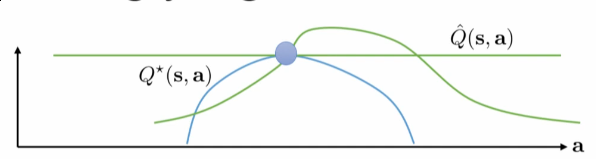
\includegraphics[width=0.5\textwidth]{figures/2020-07-16-000546_596x159_scrot.png}
\end{center}
\end{itemize}

\subsubsection{Imitación como una función de pérdida auxiliar}%
\label{ssub:imitación_como_una_función_de_pérdida_auxiliar}

El objetivo de la imitación es: $\sum_{(s,a)\in D_{demo}} \log\pi_\theta(a|s)$.

El objetivo RL es: $E_{\pi_\theta}[r(s,a)]$.

Por lo que se puede crear un objetivo híbrido:
 \begin{align}
E_{\pi_\theta}[r(s,a)] + \lambda \sum_{(s,a)\in D_{demo}} \log\pi_\theta(a|s)
\end{align}

Los problemas de esto son:
\begin{itemize}
    \item Se tiene un hiperparámetro más: $\lambda$.
    \item El diseño del objetivo necesita mucha atención
    \item El algoritmo se vuelve dependiente al problema que se quiere resolver.
\end{itemize}
